\documentclass[11pt]{article}
\usepackage{geometry}                % See geometry.pdf to learn the layout options. There are lots.
\geometry{letterpaper}                   % ... or a4paper or a5paper or ... 
%\geometry{landscape}                % Activate for for rotated page geometry
%\usepackage[parfill]{parskip}    % Activate to begin paragraphs with an empty line rather than an indent
\usepackage{graphicx}
\usepackage{amssymb}
\usepackage{epstopdf}
\DeclareGraphicsRule{.tif}{png}{.png}{`convert #1 `dirname #1`/`basename #1 .tif`.png}

\title{Single Higgs backgrounds for $HH\to4b$}
\begin{document}
\maketitle

\begin{table}[htp]
\begin{center}
\begin{tabular}{|c|c|c|c|c|}
\hline
Sample & LO & NLO & K & Ref\\
\hline\hline
$ZH$ (13 TeV) & $6.468 \cdot 10^{-1}$ pb & $ 7.674 \cdot 10^{-1}$ pb & 1.186 & \cite{Alwall:2014hca}\\
$ttH$ (13 TeV) & $3.579 \cdot 10^{-1}$ pb & $4.608 \cdot 10^{-1}$ pb & 1.287 &  \cite{Alwall:2014hca}\\
$bbH$ (13 TeV) &  $4.983 \cdot 10^{-1}$ pb & $6.085 \cdot 10^{-1}$ pb & 1.221 & \cite{Alwall:2014hca}\\
\hline
\end{tabular}
\end{center}
\label{HK}
\caption{NLO K-factors for single Higgs backgrounds.}
\end{table}%

\begin{table}[htp]
\begin{center}
\begin{tabular}{|c|c|c|c|c|}
\hline
Sample & Decay & BF & Ref\\
\hline\hline
$ZH$ & ($Z\to b\bar{b}$)($H\to b\bar{b}$) & 0.0861 & \cite{Agashe:2014kda}\\
$ttH$ & $(W\to q\bar{q})^2$($H\to b\bar{b}$) & 0.259 & \cite{Agashe:2014kda}\\
$bbH$ & $H\to b\bar{b}$ & 0.57 & \cite{Agashe:2014kda} \\
\hline
\end{tabular}
\end{center}
\label{HBF}
\caption{Branching fractions for single Higgs backgrounds.}
\end{table}%

\begin{table}[htp]
\begin{center}
\begin{tabular}{|c|c|c|c|}
\hline
Sample & Boosted (fb) & Intermediate (fb) & Resolved (fb) \\
\hline\hline
$ZH$ & $2.014\cdot 10^{-2}$ & $1.208\cdot 10^{-1}$ & $7.490\cdot 10^{-1}$ \\
$ttH$ & $5.058\cdot 10^{-2}$ & $6.325\cdot 10^{-3}$ & $4.054\cdot 10^{-1}$ \\
$bbH$ & $2.282\cdot 10^{-3}$ & $5.548\cdot 10^{-3}$ & $2.609\cdot 10^{-1}$\\
\hline\hline
$HH$ & $3.556\cdot 10^{-1}$  & $2.238\cdot 10^{-1}$ &  $1.237\cdot 10^{0}$ \\
QCD &  $2.533\cdot 10^{2}$ & $1.771\cdot 10^{2}$ & $4.866\cdot 10^{3}$ \\
\hline
\end{tabular}
\end{center}
\label{HBF}
\caption{ Results of running the OHH4b analysis code over the single Higgs background samples (noPU, pre-MVA). The numbers here are the cross sections remaining in the various channels and topologies after all analysis cuts. Also given for comparison are the post-analysis cross sections for the diHiggs signal and QCD background.}
\end{table}%

\begin{figure}
\begin{center}
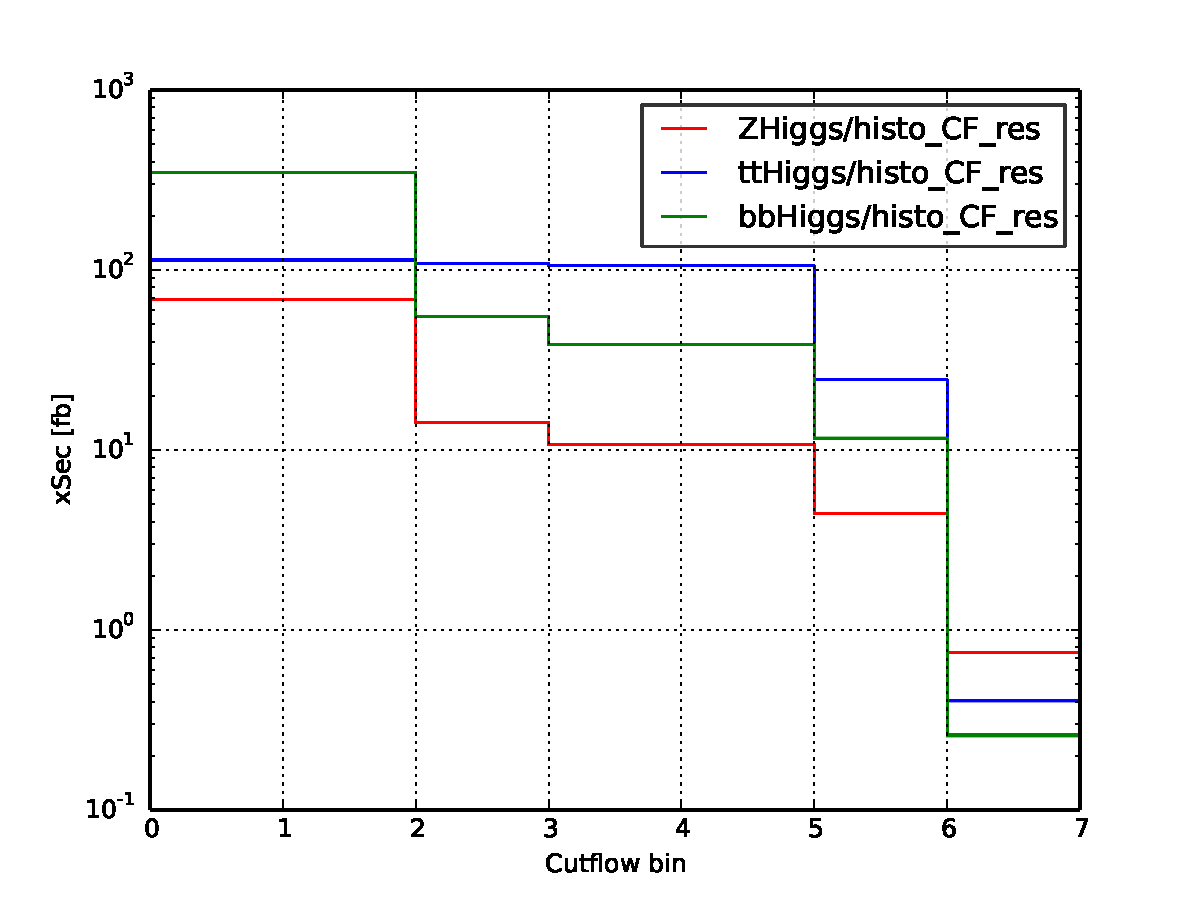
\includegraphics[width=0.45\textwidth]{plots/res.pdf}
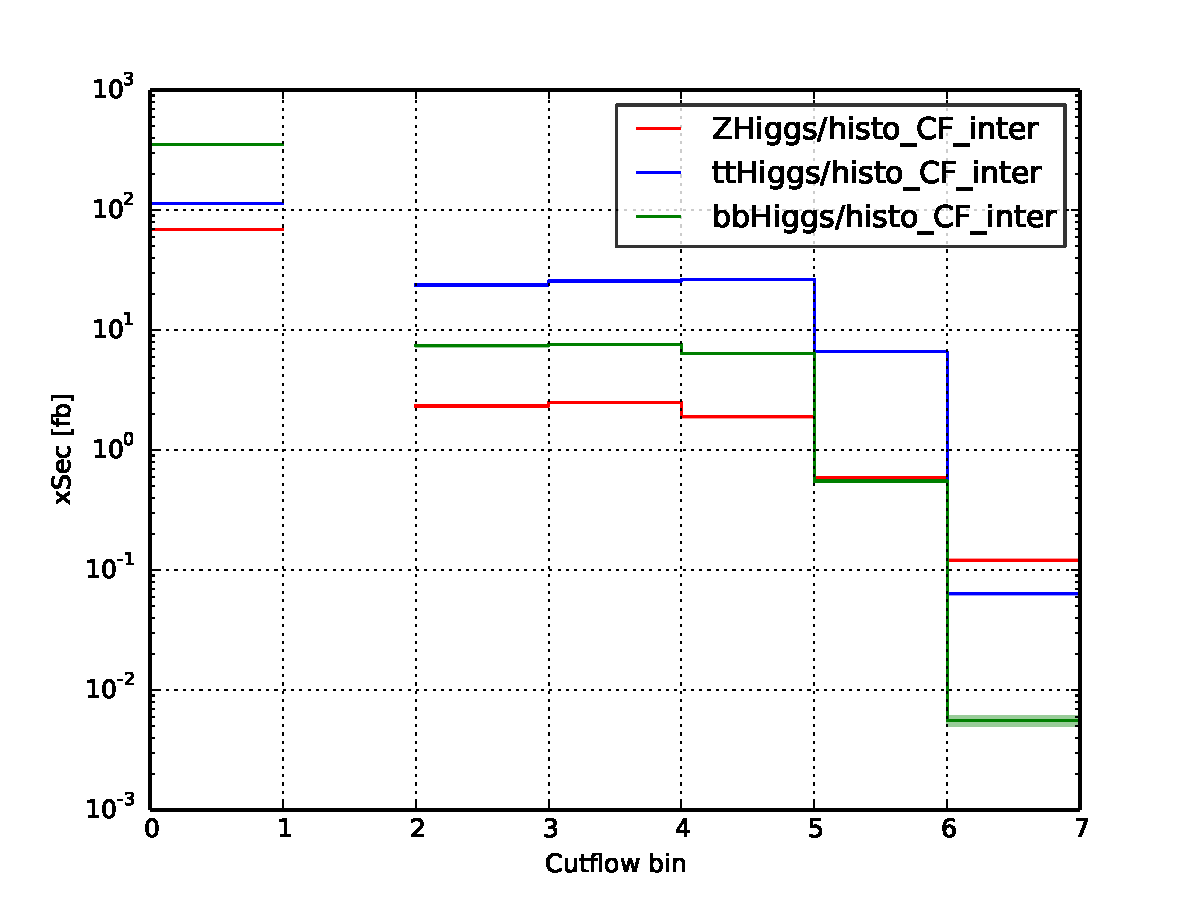
\includegraphics[width=0.45\textwidth]{plots/inter.pdf}
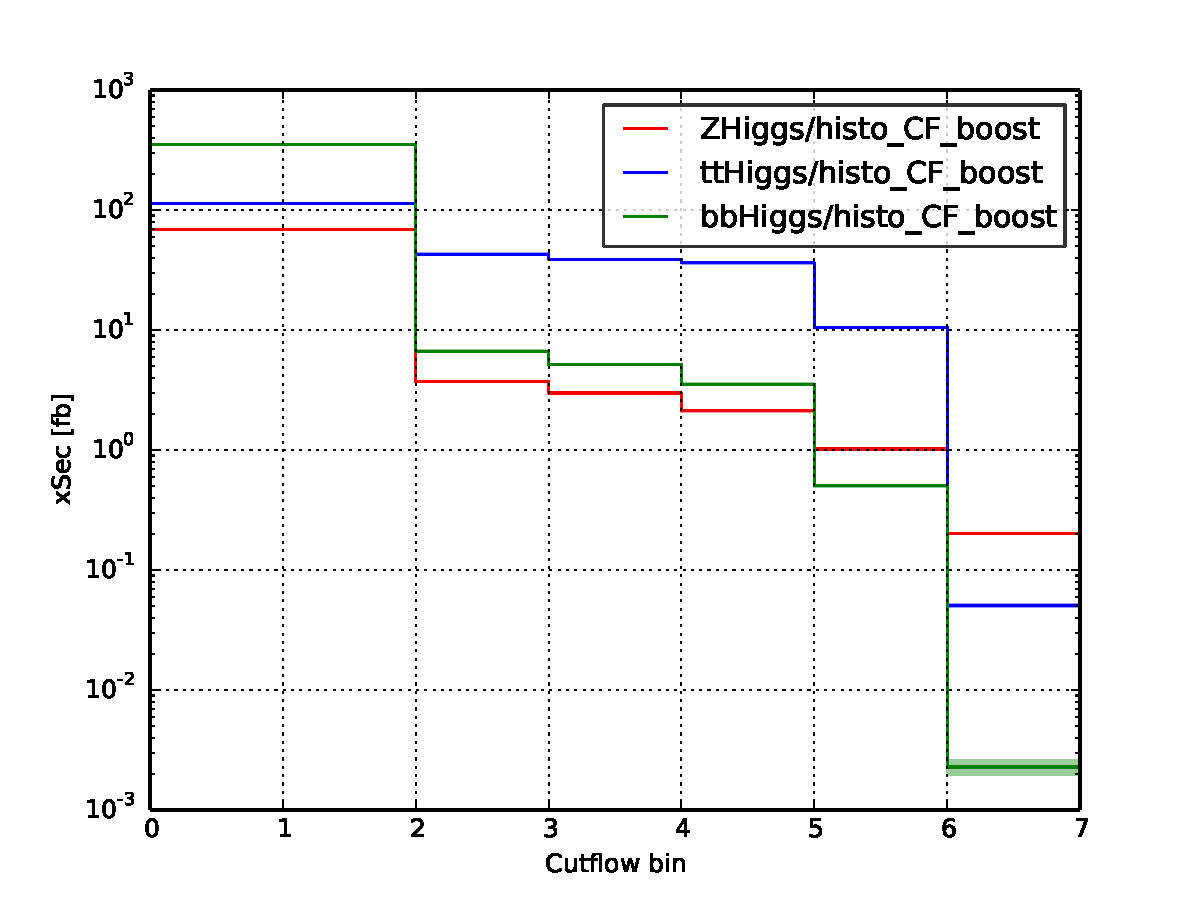
\includegraphics[width=\textwidth]{plots/boost.pdf}
\caption{Cutflows for the resolved (top-left), intermediate (top-right) and boosted (bottom) analyses of single Higgs backgrounds.}
\end{center}
\end{figure}


\begin{thebibliography}{9}

\bibitem{Alwall:2014hca}
  J.~Alwall {\it et al.},
  ``The automated computation of tree-level and next-to-leading order differential cross sections, and their matching to parton shower simulations,''
  JHEP {\bf 1407} (2014) 079
  doi:10.1007/JHEP07(2014)079
  [arXiv:1405.0301 [hep-ph]].
  %%CITATION = doi:10.1007/JHEP07(2014)079;%%
  %759 citations counted in INSPIRE as of 01 Mar 2016
  
\bibitem{Agashe:2014kda}
  K.~A.~Olive {\it et al.} [Particle Data Group Collaboration],
  %``Review of Particle Physics,''
  Chin.\ Phys.\ C {\bf 38} (2014) 090001.
  doi:10.1088/1674-1137/38/9/090001
  %%CITATION = doi:10.1088/1674-1137/38/9/090001;%%
  %3117 citations counted in INSPIRE as of 01 Mar 2016
  
\end{thebibliography}


%\subsection{}



\end{document}  